\chapter{Receiver Testing}

\section{Introduction}
  \subsection{Order of Components}


\section{Load Stabilisation}
  \subsection{Cryocontrol}
\subsection{Bobbin Redesign}
\subsection{Temperature Sensor}


\section{RF and IF Band Definitions}




\begin{figure}[ht]
 \centering
\subfloat[Full Band measured by changing to 4GHz LO. This shows the low side rolloff. The steep slope after 1GHz is due to the power splitter frequency response.]{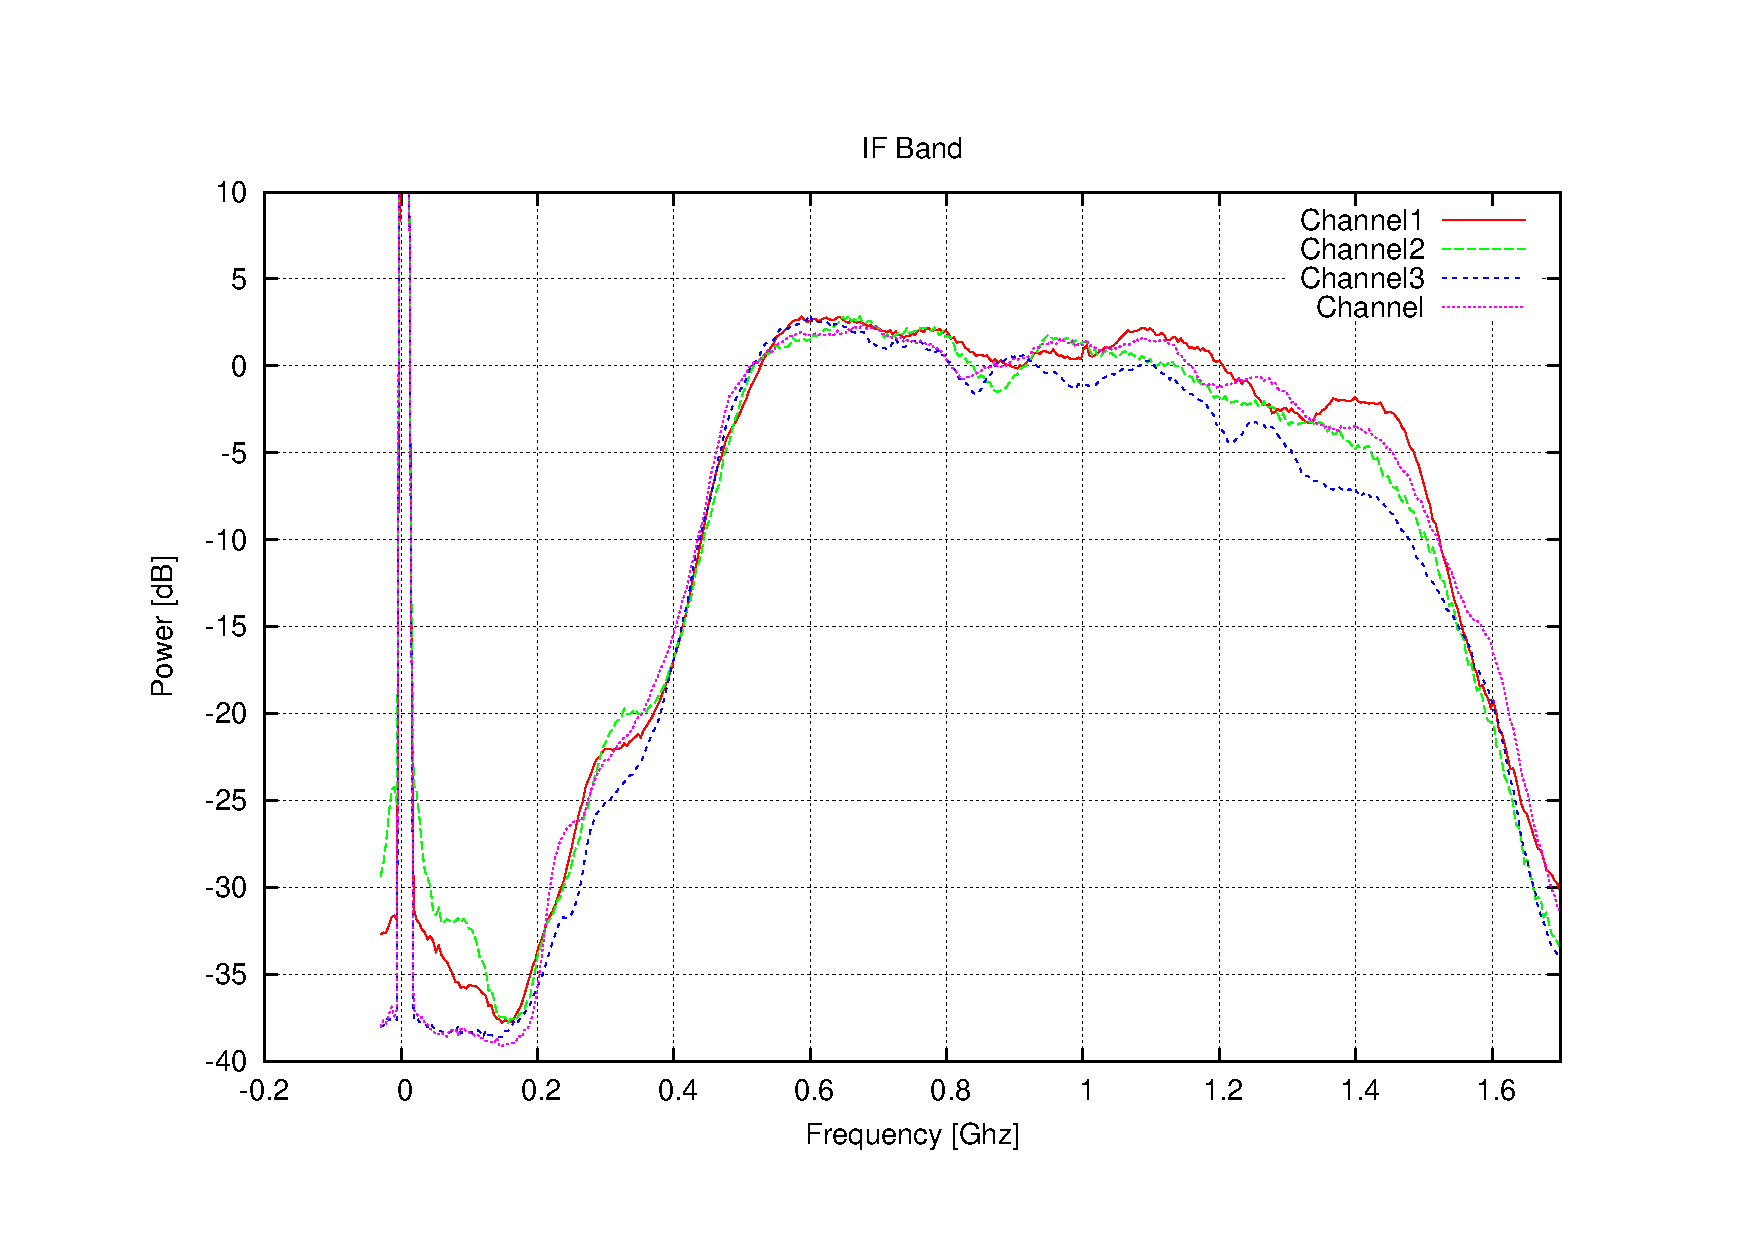
\includegraphics[width=0.4\textwidth]{./images/digitalReceiver/BandPassPlots/IFBandPass4GHzLO.pdf}\label{fig:IFBandDefinitions4GHz}}
\hspace{0.2cm}
\subfloat[The two digitised bands, DC$\rightarrow$500~MHz and 500$\rightarrow$1000~MHz]{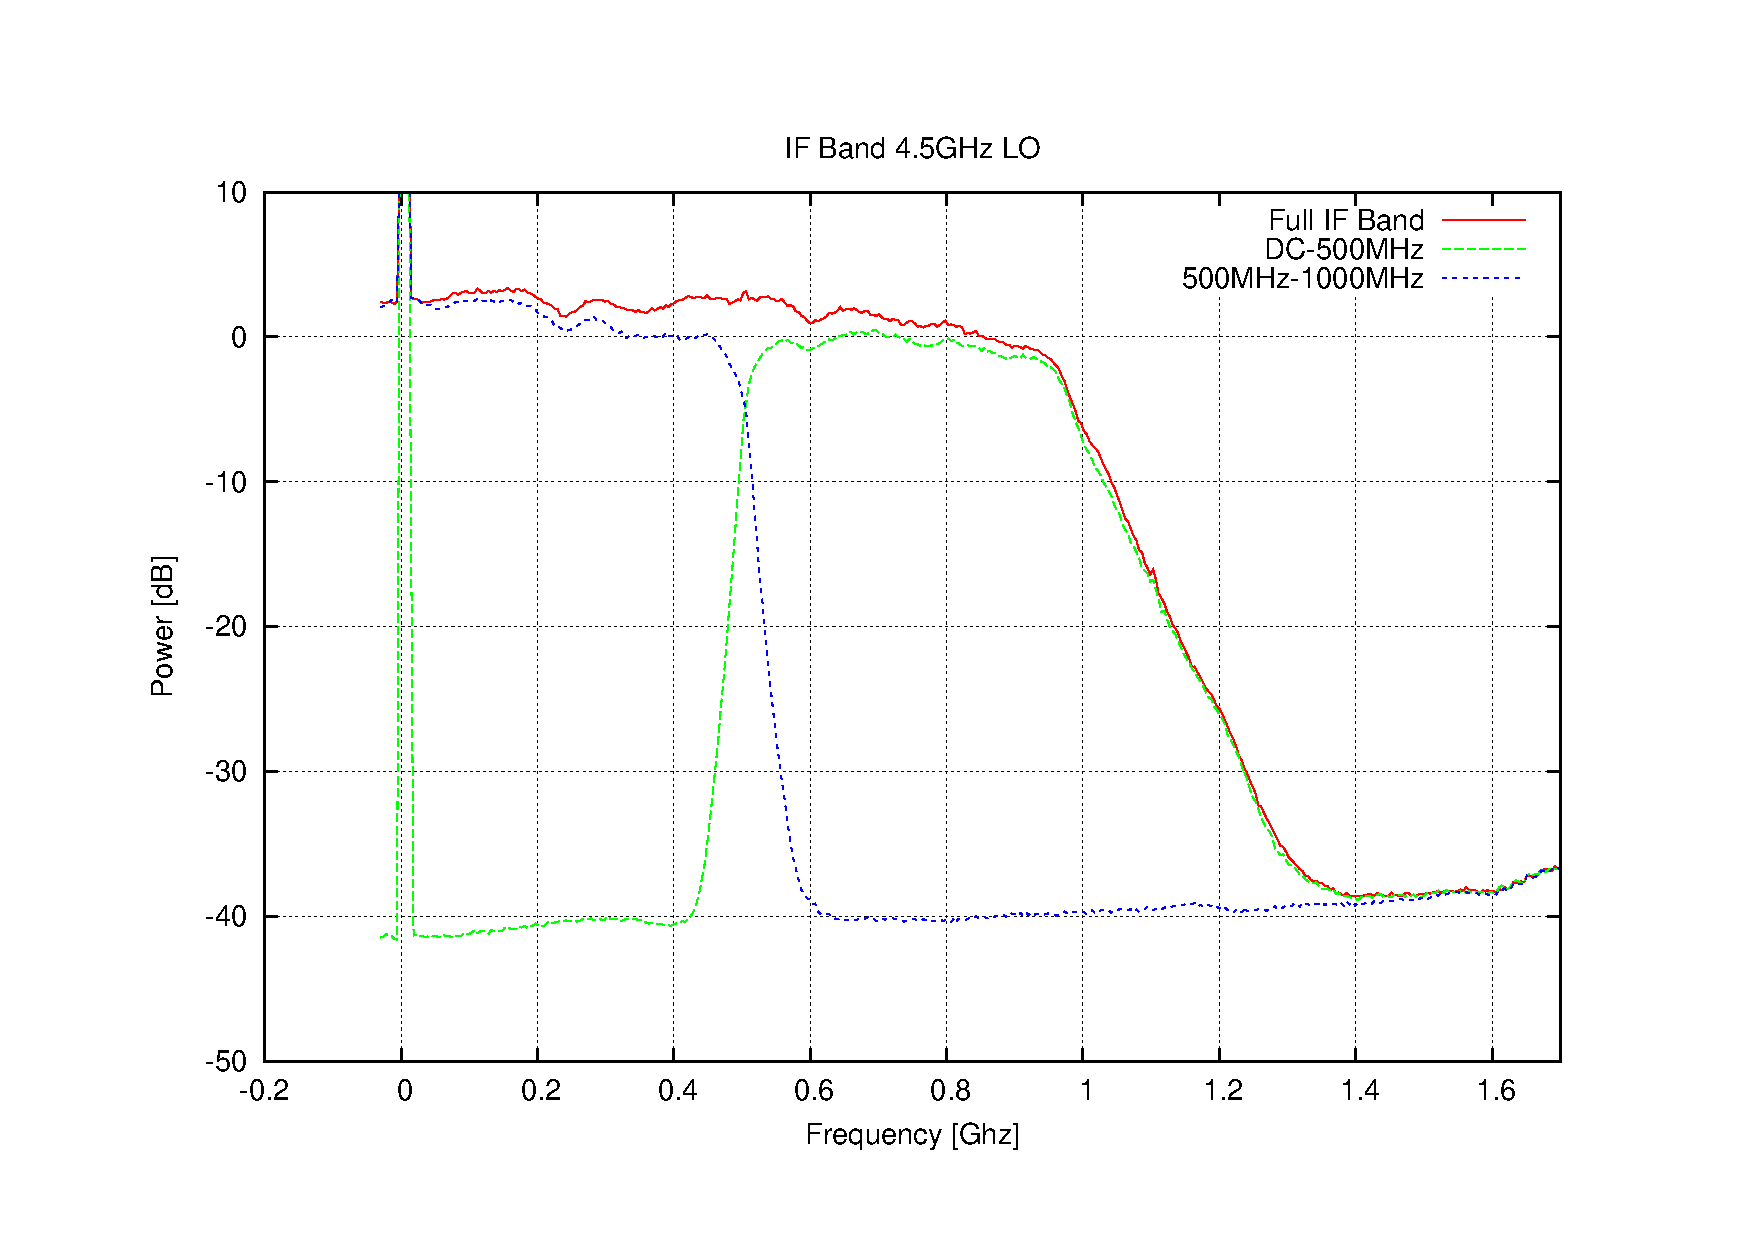
\includegraphics[width=0.4\textwidth]{./images/digitalReceiver/BandPassPlots/IFBandPass4_5GHzLO.pdf}\label{fig:IFBandDefinitions4.5GHz}}
\caption{Measurements of the IF Bands digitised by the iADC}
\label{fig:IFBandDefinitions}


\end{figure}




  \subsection{System Temperature}

\section{2-20GHz Amplifier System Tests}
  \subsection{System Temperature}

\section{DC-4GHz Amplifiers}

\subsection{Wideband Capacitors}

\subsection{Wideband Biasing Choke}

\section{Horn Tests}
  \subsection{Anechoic Chamber Measurements}


\section{Full System Tests}
  \subsection{Low Noise Amplifiers (LNA)}

\subsection{Cold Component Tests} 

\section{Design Improvements over Northern Frontend}

  \subsection{SuperSMA connectors}

  \subsection{Redesign RF route}

  \subsection{Thermal decoupling of temperature Load}


  


